\subsection{Providing context: single-trial regressions of haptic and velocity at moments of spatio-temporal asynchrony}
Figure \ref{st_ersp} B shows betas from single-trial regression including a baseline vector, whether physics were in part rendered through haptic feedback, hand velocity at the moment of spatio-temporal asynchrony, their interaction as well as the time elapsed since the object spawned. Low alpha-band during the baseline interval preceding object spawn positively impacted low-alpha band power preceding and following the object selection event ($t_{16} = 2.95, P = 0.003$ at 200 ms and 9 Hz post event), see \ref{st_ersp} B, C first column. Further, baseline beta-band power between 19-27 Hz impacted post event beta-band power in scattered clusters at 500 and 1000 ms post event. As expected, 50 Hz during baseline positively impacted 50 Hz band power during the trial hinting at the presence of line noise in some if not all independent components comprising the cluster.
% make sure the names are congruent throughout paper
% idea: separate RT measure in RT and 'action time' -> the time from spawn to movement start
% velocity -> slack in the system
% RT -> generelle "kognitive Aufmerksamkeit"
\begin{figure}[t]
  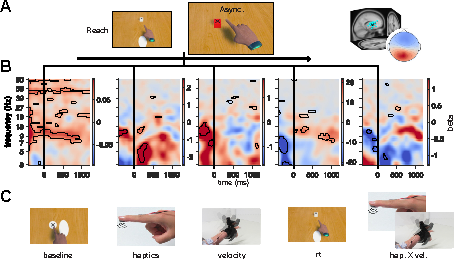
\includegraphics[width=\textwidth]{figures/fig4_ersp_single_trial_short.pdf}
  \caption{\textbf{A} Moment of spatio-temporal asynchrony. \textbf{B} Multiple regression coefficients, betas. Black lines enclose areas of significant regions containing at least 10 pixels below P = .05 calculated using permutation t-tests. For visualization, time-frequency maps were smoothed with a Gaussian (width = 1.5).} \textbf{C} Predictors.
  \label{st_ersp}  
\end{figure}
With increasing time elapsed between object spawn and object selection, reaction time, alpha-band power increased following visuo-spatial asynchronous object selection ($t_{16} = 1.96, P = 0.03$ at 250 ms and 12 Hz post event), see \ref{st_ersp} B, C fourth column. Preceding the event, reaction time negatively impacted a theta-band burst ($t_{16} = -2.91, P = 0$ at -200 ms and 7 Hz pre event). The two \textit{contextual} sensory predictors haptics and hand velocity at the moment of object selection as well as their interaction exhibited differential influence compared with baseline and reaction time predictors. Enabling vibrotactile stimulation increased theta-band power immediately following the moment of object selection ($t_{16} = 2.52, P = 0.02$ at 180 ms and 5 Hz post event). Further, enabling vibrotactile stimulation increased high alpha-band activity in a similar time window ($t_{16} = 2.58, P = 0.02$ at 180 ms and 12 Hz post event). Both enabling vibrotactile stimulation and increasing hand velocity increased alpha-band activity preceding object selection, exemplary for hand velocity ($t_{16} = 3.43, P = 0.003$ at -200 ms and 12 Hz pre event). Besides small, scattered clusters, hand velocity did not impact event-related spectral activity as a main effect. However, increasing hand velocity decreased theta-band power in a burst immediately succeeding object selection ($t_{16} = -2.05, P = 0.04$ at 180 ms and 4 Hz). Further, pre-event interaction effects indicated a decrease around the alpha-band with increasing hand velocity in vibrotactile trials only.